\section{What each stage contributes}
\label{sec:analysis}
Figure~\ref{fig:stages} shows the pipeline on images chosen by a fixed rule, and Table~\ref{tab:progression} measures each decision against the previous one in the same run. The CA seed marks the class but is incomplete. Coarse SA spreads it over the object, fine SA restores the outline, and DenseCRF aligns it with edges. This section explains each step in turn.

\begin{figure*}[t]
\centering
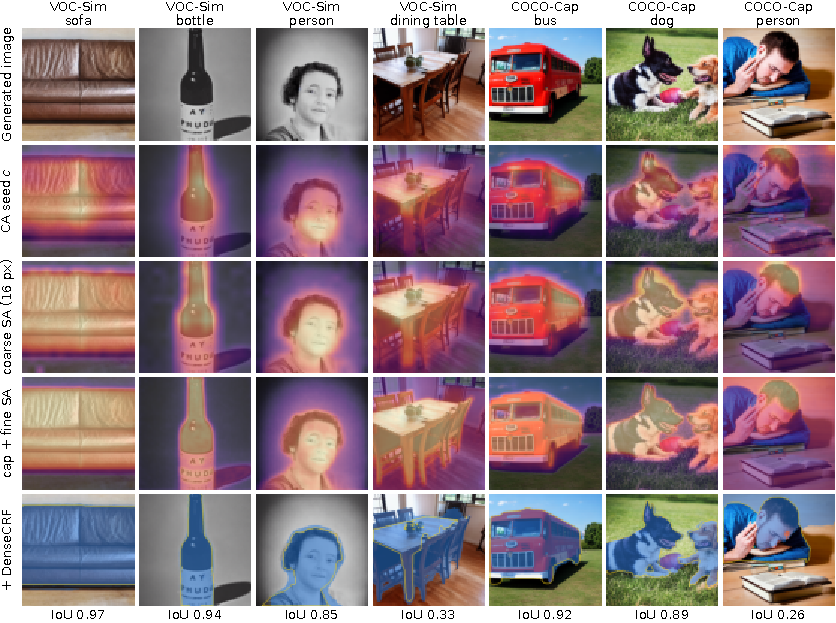
\includegraphics[width=\textwidth]{figures/pipeline_c2f.pdf}
\caption{\textbf{From seed to mask.} Columns are chosen by a fixed rule, without inspecting any image: the VOC-Sim classes at the best, upper-third, lower-third and worst class IoU of the final pipeline, and the COCO-Cap classes at the best, median and worst, each shown by its median-IoU image. Rows: generated image; A3 CA seed $c$; after coarse 16-pixel SA ($r$); after the cap and fine 64-pixel SA ($y$); final mask after DenseCRF (blue) with the annotation outline (yellow). The worst columns show the two characteristic failures: SA groups the dining table with its chairs, and a weak person seed spreads to the pillow.}
\label{fig:stages}
\end{figure*}

\begin{table}[t]
\centering
\footnotesize\setlength{\tabcolsep}{2.4pt}
\begin{tabular}{@{}ccccccc|ccc@{}}
\toprule
\rotatebox{90}{no 32-px CA} & \rotatebox{90}{SA 64 px} & \rotatebox{90}{2 passes} & \rotatebox{90}{DenseCRF} & \rotatebox{90}{calls 10--20} & \rotatebox{90}{SA-guided weights} & \rotatebox{90}{coarse-to-fine + cap} & VOC & $\Delta$ & COCO \\
\midrule
 & & & & & & & .665 & & -- \\
$\checkmark$ & & & & & & & .691 & +.026 & -- \\
$\checkmark$ & $\checkmark$ & & & & & & .789 & +.033$^a$ & -- \\
$\checkmark$ & $\checkmark$ & $\checkmark$ & & & & & .800 & +.012 & .625 \\
$\checkmark$ & $\checkmark$ & $\checkmark$ & $\checkmark$ & & & & .813 & +.014 & .637 \\
$\checkmark$ & $\checkmark$ & $\checkmark$ & $\checkmark$ & $\checkmark$ & & & .817 & +.004 & .644 \\
$\checkmark$ & $\checkmark$ & $\checkmark$ & $\checkmark$ & $\checkmark$ & $\checkmark$ & & .823 & +.006 & .662 \\
$\checkmark$ & $\checkmark$ & $\checkmark$ & $\checkmark$ & $\checkmark$ & $\checkmark$ & $\checkmark$ & \textbf{.829} & +.006 & \textbf{.696} \\
\bottomrule
\end{tabular}
\caption{\textbf{The pipeline, one decision at a time.} VOC: OOF mIoU; $\Delta$: gain over the previous row \emph{measured in the same run} (same generated images); COCO-Cap: VOC-frozen transfer. The first three rows come from early one-axis screens at a fixed threshold 0.45 (CA only, then one SA pass); $^a$against one pass through all sixteen SA modules (.756). Later rows select thresholds inside the training folds. Runs differ by at most 0.0003 on a shared reference.}
\label{tab:progression}
\end{table}


\subsection{Seed: which CA scales, and how to weight them}
\label{sec:seed}
CA is the only source of class identity, so the seed sets an upper bound on everything downstream. Table~\ref{tab:seed} (top) shows that no single CA scale suffices. The 16-pixel modules are the strongest alone, 8-pixel modules localize coarsely, and 64-pixel CA alone is nearly unusable (0.17 mIoU) because it fires on texture (see the supplementary seed gallery). The 32-pixel modules hurt in every combination: removing them raises OOF mIoU from 0.665 to 0.691 in 4/5 folds (paired $+0.022$, CI $[+0.015,+0.029]$). Restricting CA heads or calls did not survive once crossed with this choice.

Uniform averaging still lets the noisy 64-pixel modules contribute five of eleven votes. The A3 weights of Eq.~\eqref{eq:a3} learn nothing, yet they shift 84\% of the weight to the 8- and 16-pixel modules, most strongly at early, noisy calls (supplementary material). Interestingly, A3 \emph{lowers} the CA-only score (0.714$\to$0.705) but raises the final mask from 0.817 to 0.823 (4/5 folds) and COCO-Cap from 0.644 to 0.662 (Table~\ref{tab:seed}, bottom). A seed is good if SA can propagate it, not if it is the best mask on its own. This is the first sign that coarse structure is the right base.

\begin{table}[t]
\centering
\footnotesize\setlength{\tabcolsep}{3.2pt}
\begin{tabular}{@{}cccc|cc@{}}
\toprule
\multicolumn{4}{c|}{CA resolutions (px)} & \multicolumn{2}{c}{CA seed only, VOC-Sim}\\
8 & 16 & 32 & 64 & mIoU@.45 & AP \\
\midrule
$\checkmark$ & & & & .563 & .846 \\
 & $\checkmark$ & & & .649 & .906 \\
 & & $\checkmark$ & & .300 & .822 \\
 & & & $\checkmark$ & .173 & .560 \\
$\checkmark$ & $\checkmark$ & $\checkmark$ & $\checkmark$ & .666 & .922 \\
$\checkmark$ & $\checkmark$ & & & .693 & .917 \\
$\checkmark$ & $\checkmark$ & & $\checkmark$ & \textbf{.696} & .913 \\
\bottomrule
\end{tabular}\\[3pt]
\begin{tabular}{@{}lccc@{}}
\toprule
Module weights $w_{t,m}$ & CA only & + propagation, R2 & COCO \\
\midrule
uniform & .714 & .817 & .644 \\
A3 (SA agreement, Eq.~\ref{eq:a3}) & .705 & \textbf{.823} & \textbf{.662} \\
\bottomrule
\end{tabular}
\caption{\textbf{Building the semantic seed.} \emph{Top:} CA-only mIoU at threshold 0.45 and average precision for resolution subsets (all calls and heads; full VOC-Sim, descriptive). Each scale alone is weak and 64-px CA is nearly unusable alone, but 8, 16 and 64 px are complementary; dropping the 32-px modules raises out-of-fold (OOF) mIoU from 0.665 to 0.691 (4/5 folds). \emph{Bottom:} module weighting, forced OOF in one run (MID-P2 propagation of Sec.~\ref{sec:exp}). A3 lowers the CA-only score yet improves the final mask in 4/5 folds and on COCO-Cap: it favours modules whose spatial structure SA can propagate.}
\label{tab:seed}
\end{table}


\subsection{Envelope: why start from coarse self-attention}
\label{sec:envelope}
SA at different scales groups pixels differently. Figure~\ref{fig:scales} (left, middle) compares propagating the same seed through 16-pixel SA only, 64-pixel SA only, and from 16 to 64 pixels. Coarse SA keeps recall high as the threshold rises (0.73 at $\tau{=}0.70$ on VOC-Sim, against 0.61 for fine SA), because it assigns whole regions, not textures, to the object. Its precision is low, however: blocks along the boundary are all-or-nothing, and alone it scores only 0.723 OOF. Fine SA is precise but loses object parts at high thresholds. Going from coarse to fine keeps most of the coarse recall at nearly fine precision. On cluttered COCO-Cap, where fine SA leaks into look-alike textures, it already beats fine-only propagation (0.687 vs.\ 0.660 frozen). On VOC-Sim, however, it falls short (0.802 vs.\ 0.810 OOF). The coarse envelope is useful, but on its own it lets the finer levels claim too much. The cap addresses this.

\begin{figure*}[t]
\centering
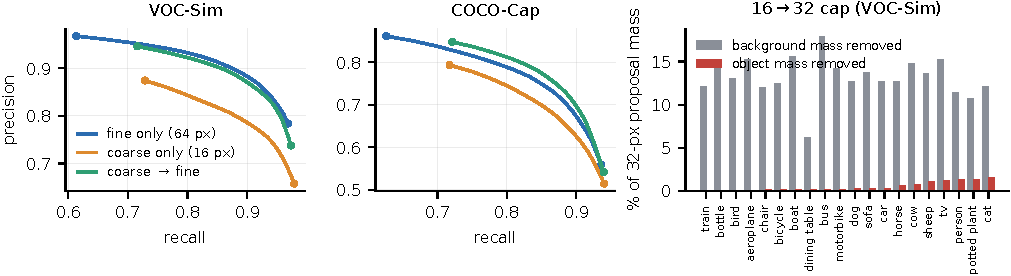
\includegraphics[width=\textwidth]{figures/scale_profiles.pdf}
\caption{\textbf{Coarse SA gives the envelope; the cap trims only background.} \emph{Left, middle:} pooled precision and recall over the threshold grid (0.30 at the high-recall end to 0.70) for one seed propagated by 64-pixel SA only, 16-pixel SA only, or 16$\to$64 pixels (two passes per level, same run). Coarse SA keeps recall at high thresholds and coarse-to-fine combines it with fine precision. \emph{Right:} share of the 32-pixel proposal's mass that the cap removes inside the annotated object (red) and in the background (grey), per VOC-Sim class (ground truth is used only for this diagnostic). Overall 13\% of background mass and 0.5\% of object mass are removed.}
\label{fig:scales}
\end{figure*}

\subsection{Detail within the envelope: cap, not conservation}
\label{sec:cap}
How strongly should the coarse level constrain the next? Table~\ref{tab:hierarchy} answers this in one run. The plain hierarchy (no constraint) loses to fine-only propagation on VOC-Sim. Forcing exact mass conservation at both transitions is far worse (0.759 raw, $-$5 points). Conservation at $16\to32$ alone, or conservation followed by fine completion, stays below fine-only after R2. The one-sided cap is the only variant that beats both fine-only propagation and the plain hierarchy in every fold: 0.830 after R2, $+0.012$ over the plain hierarchy (CI $[+0.006,+0.013]$), with 0.697 on COCO-Cap. A second cap at $32\to64$ adds nothing, which confirms that fine SA should refine boundaries freely. Re-adding completion on top of the cap re-introduces false positives and erases the COCO-Cap gain.

Why does the one-sided form work? The coarse parent is a reliable \emph{upper bound} on where the object can be, but not a reliable lower bound. The cap binds in 58\% of $2\times2$ groups yet removes only 7.6\% of the proposal mass. As Fig.~\ref{fig:scales} (right) shows, that mass is almost all background: 13\% of the background mass but 0.5\% of the object mass, and at most 1.6\% for any class. Conservation instead makes children inherit the budget of every parent, including parents that the blurry coarse map wrongly made confident, and it must spend that budget somewhere. Figure~\ref{fig:cap} shows the effect. Conservation distorts the mask wherever a parent's budget is wrong (COCO cat: IoU 0.58, against 0.81 with the cap), whereas the cap removes mass only where the coarse level disagrees.

\begin{table*}[t]
\centering
\footnotesize\setlength{\tabcolsep}{4.2pt}
\begin{tabular}{@{}l|ccc|ccc|cc|ccc@{}}
\toprule
& \multicolumn{3}{c|}{SA levels} & \multicolumn{3}{c|}{transition $16\!\rightarrow\!32$ / $32\!\rightarrow\!64$} & & & \multicolumn{3}{c}{mIoU}\\
Variant & 16 & 32 & 64 & conserve ($=$) & cap ($\le$) & cap $32\!\rightarrow\!64$ & completion & wins & VOC raw & VOC + R2 & COCO + R2 \\
\midrule
fine only (FINE-P2) & & & $\checkmark$ & & & & & -- & .8098 & .8231 & .6622 \\
plain hierarchy & $\checkmark$ & $\checkmark$ & $\checkmark$ & & & & & 1/5 & .8061 & .8184 & .6925 \\
\midrule
conservation at $16\!\rightarrow\!32$ & $\checkmark$ & $\checkmark$ & $\checkmark$ & $16\!\rightarrow\!32$ & & & & 2/5 & .8034 & .8185 & .7038 \\
conservation at $32\!\rightarrow\!64$ & $\checkmark$ & $\checkmark$ & $\checkmark$ & $32\!\rightarrow\!64$ & & & & 0/5 & .7894 & .8135 & .7022 \\
conservation at both & $\checkmark$ & $\checkmark$ & $\checkmark$ & both & & & & 0/5 & .7592 & .7917 & .6851 \\
relaxed conservation ($\rho{=}.5$) & $\checkmark$ & $\checkmark$ & $\checkmark$ & both, $\rho{=}.5$ & & & & 1/5 & .7926 & .8149 & .7059 \\
conservation + completion & $\checkmark$ & $\checkmark$ & $\checkmark$ & both & & & $\checkmark$ & 2/5 & .8037 & .8204 & \textbf{.7063} \\
\midrule
\textbf{one-sided cap (ours)} & $\checkmark$ & $\checkmark$ & $\checkmark$ & & $\checkmark$ & & & \textbf{5/5} & \textbf{.8157} & \textbf{.8304} & .6966 \\
cap at both transitions & $\checkmark$ & $\checkmark$ & $\checkmark$ & & $\checkmark$ & $\checkmark$ & & 4/5 & .8151 & .8290 & .6964 \\
cap + completion & $\checkmark$ & $\checkmark$ & $\checkmark$ & & $\checkmark$ & & $\checkmark$ & 3/5 & .8131 & .8209 & .6647 \\
\bottomrule
\end{tabular}
\caption{\textbf{How the coarse level should constrain the finer one.} All rows share one generation of the 490 VOC-Sim and 707 COCO-Cap images, the A3 seed and SA calls 10--20. VOC columns are forced OOF mIoU; wins counts the held-out folds in which a row beats FINE-P2 after R2; COCO-Cap uses the VOC-frozen threshold. \emph{Conserve} forces every $2{\times}2$ child group to carry exactly its parent's mass (closed-form KL projection); \emph{cap} only removes mass above the parent (Eq.~\ref{eq:cap}). \emph{Completion} re-adds positive fine-SA residuals. Forcing parent mass onto children loses up to 5 VOC points; capping is the only change that beats both the fine-only and the plain hierarchy in every fold (vs.\ plain hierarchy: $+0.012$ after R2, paired 95\% CI $[+0.006,+0.013]$).}
\label{tab:hierarchy}
\end{table*}


\begin{figure}[t]
\centering
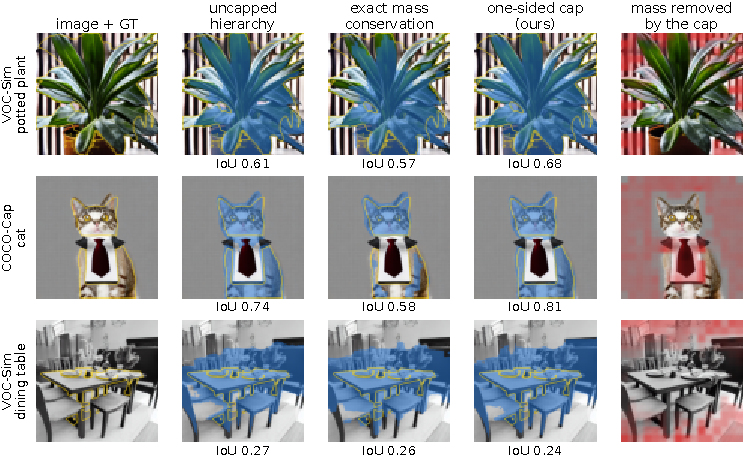
\includegraphics[width=\columnwidth]{figures/cap_mechanism.pdf}
\caption{\textbf{Cap versus conservation.} Images at the 95th percentile of the cap's IoU gain over the plain hierarchy on VOC-Sim and COCO-Cap, and at the 5th percentile on VOC-Sim (fixed rule). Masks at each variant's VOC-selected threshold. Right: mass removed by the cap (red). The cap removes background mass that the coarse level does not support; conservation spreads mass into it. When the coarse level groups the table with its chairs (bottom), no variant can separate them.}
\label{fig:cap}
\end{figure}

\subsection{Boundary: what DenseCRF adds}
\label{sec:refine}
SA works on a 64-pixel grid, so even a good map has blocky, slightly dilated borders (Fig.~\ref{fig:crf}). DenseCRF uses the image itself: the pairwise kernel of Eq.~\eqref{eq:crf} prefers equal labels for nearby pixels of similar colour, so mask boundaries snap to edges. With fixed parameters it improves 278 VOC-Sim images and worsens 97, and raises mIoU by 0.013 (Table~\ref{tab:refine}). Its effect depends on what it is given. On fine-only maps it mainly adds recall and barely helps COCO-Cap ($+0.002$, with 243 images worse). On capped coarse-to-fine maps it raises precision, helps COCO-Cap six times more ($+0.014$, 18 of 20 classes), and turns 427 images better against 105 worse. Once the cap has removed far-away mass, the remaining errors lie near boundaries, where appearance is informative. DenseCRF fails when appearance misleads: a chair's thin legs against a similar background (Fig.~\ref{fig:crf}, bottom).

\begin{table}[t]
\centering
\footnotesize\setlength{\tabcolsep}{2.6pt}
\begin{tabular}{@{}cc|ccc|ccc@{}}
\toprule
\multicolumn{2}{c|}{} & \multicolumn{3}{c|}{VOC-Sim} & \multicolumn{3}{c}{COCO-Cap}\\
\shortstack{coarse-\\to-fine} & CRF & mIoU & P / R & img $\uparrow$/$\downarrow$ & mIoU & P / R & img $\uparrow$/$\downarrow$ \\
\midrule
 & & .811 & .880 / .904 & & .660 & .708 / .882 & \\
 & $\checkmark$ & .824 & .883 / .916 & 291/132 & .662 & .703 / .889 & 354/243 \\
$\checkmark$ & & .817 & .875 / .915 & & .682 & .731 / .889 & \\
$\checkmark$ & $\checkmark$ & \textbf{.830} & \textbf{.890} / .910 & 278/97 & \textbf{.696} & \textbf{.747} / .886 & 427/105 \\
\bottomrule
\end{tabular}
\caption{\textbf{What DenseCRF adds, and why it pairs with the cap.} Full-VOC mIoU, pooled precision/recall and the number of images whose IoU rises/falls by more than 0.005 when DenseCRF is added (same run; thresholds from VOC-Sim, frozen for COCO-Cap). On fine-only maps DenseCRF mainly recovers recall and barely helps COCO-Cap ($+0.002$). On capped coarse-to-fine maps it raises precision and helps COCO-Cap six times more ($+0.014$, 18 of 20 classes): with far-away mass removed, the remaining errors lie near object boundaries, where appearance decides.}
\label{tab:refine}
\end{table}


\begin{figure}[t]
\centering
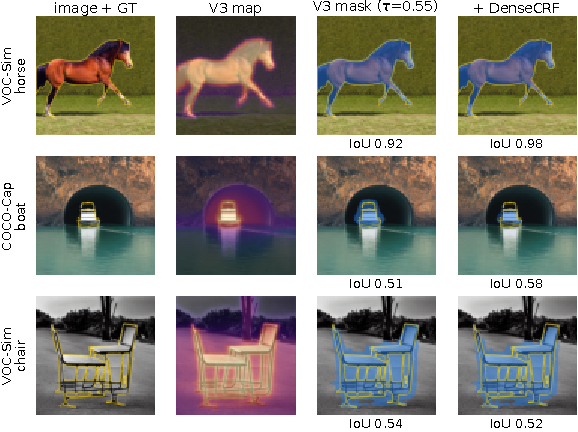
\includegraphics[width=\columnwidth]{figures/crf_effect.pdf}
\caption{\textbf{DenseCRF snaps the mask to image edges.} Images at the 90th percentile of the DenseCRF gain on VOC-Sim and COCO-Cap, and at the 10th percentile on VOC-Sim (fixed rule).}
\label{fig:crf}
\end{figure}

\subsection{What the hierarchy changes: calibration across images}
\label{sec:calibration}
The cap barely changes the \emph{ranking} of pixels within an image: raw average precision on COCO-Cap is unchanged ($-0.0006$). If each image could choose its own threshold (an oracle that uses ground truth), fine-only and coarse-to-fine maps would tie (0.896 vs.\ 0.895 after R2, Fig.~\ref{fig:threshold}). The gain lies in \emph{calibration}: after the cap, one global threshold fits many more images. Removing background mass makes small objects stand out, so the best global threshold moves from 0.425 to 0.55, and at that threshold the curve peaks higher on both benchmarks.

This also explains the one class that loses. Many sheep images are close-ups that fill 80--95\% of the frame. Sheep prefer a low threshold (0.35, the best for fine-only maps). At that threshold the capped map leaks into the surroundings, with twice the false positives of the fine-only map. At the shared threshold of 0.55, sheep IoU falls by 0.09. At a matched threshold, the capped map is actually better on sheep (0.807 vs.\ 0.778 at 0.55), and the cap removes only 1.1\% of sheep pixels. We tested six label-free per-image thresholding rules, including Otsu, two-Gaussian fits and area matching. None improved the capped pipeline, and the one that repaired sheep (matching the fine-only map's area) gave back most of the gain (supplementary material). The loss is a calibration trade-off of a single global threshold, not a failure of the propagation.

\begin{figure}[t]
\centering
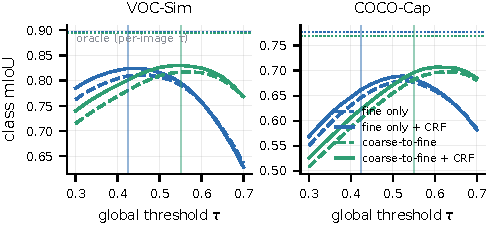
\includegraphics[width=\columnwidth]{figures/threshold_curves.pdf}
\caption{\textbf{The hierarchy improves calibration, not ranking.} Class mIoU against the global threshold for fine-only (FINE-P2) and coarse-to-fine (V3) maps, raw (dashed) and with DenseCRF (solid), on all images of one run. Vertical lines: VOC-selected thresholds (0.425 and 0.55). Dotted: per-image best threshold (oracle, uses ground truth), which ties the two maps.}
\label{fig:threshold}
\end{figure}
